\documentclass{article}
\usepackage[a4paper,margin=1in,landscape]{geometry}
\usepackage{pgfplots}
\pgfplotsset{compat=newest}
\usepackage{soul}
\usepgfplotslibrary[groupplots]
\usepgfplotslibrary{colorbrewer}

\usepackage[T1]{fontenc}
% % Palatino for main text and math
\usepackage{times}

% % Helvetica for sans serif
% % (scaled to match size of Palatino)
% \usepackage[scaled=0.90]{helvet}

% % Bera Mono for monospaced
% % (scaled to match size of Palatino)
% \usepackage[scaled=0.85]{beramono}




\begin{document}
\normalsize
% This file was created by tikzplotlib v0.9.2.
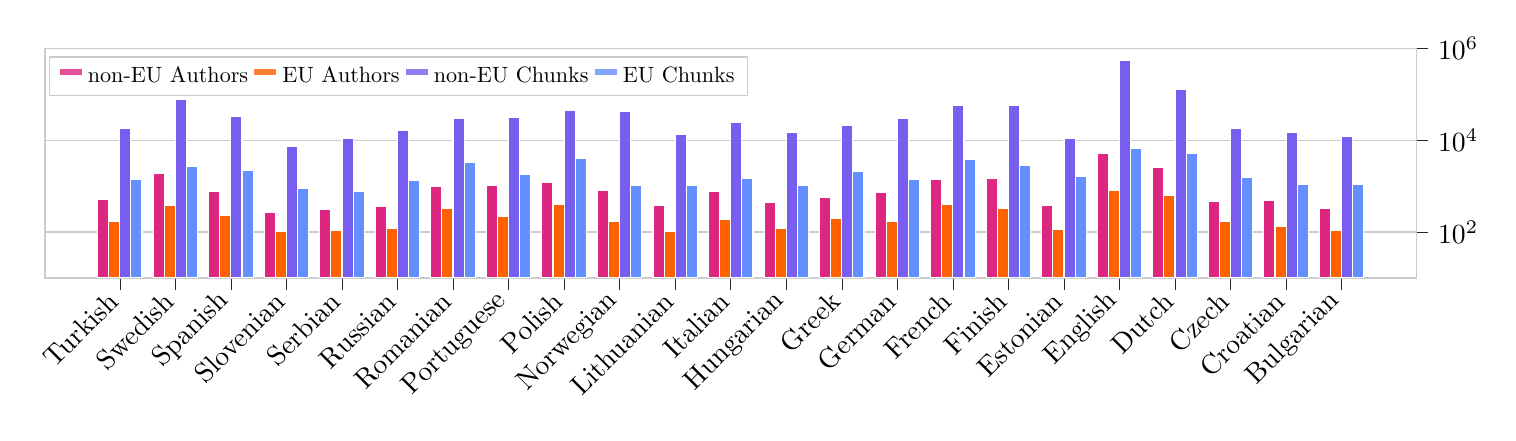
\begin{tikzpicture}

\definecolor{color0}{HTML}{648fff}
\definecolor{color1}{HTML}{785ef0}
\definecolor{color2}{HTML}{fe6100}
\definecolor{color3}{HTML}{dc267f}
\definecolor{color4}{HTML}{ffb000}
\definecolor{color5}{HTML}{000000}

% \definecolor{color0}{rgb}{0.333333333333333,0.658823529411765,0.407843137254902}
% \definecolor{color1}{rgb}{0.298039215686275,0.447058823529412,0.690196078431373}
% \definecolor{color2}{rgb}{1,0.647058823529412,0}
% \definecolor{color3}{rgb}{0.768627450980392,0.305882352941176,0.32156862745098}

\begin{axis}[
height=19cm,
width=4.5cm,
rotate around={90:(current axis.origin)},
axis line style={white!80!black},
legend cell align={left},
legend style={fill opacity=0.8, legend columns=-1, draw opacity=1, text opacity=1, draw=white!80!black, nodes={scale=0.8, transform shape}, at={(1.195,2.71)}},
tick align=outside,
xtick pos=left,
%ymajorgrids=true,
x grid style={white!80!black},
xmajorticks=true,
xtick style={color=white!15!black},
xticklabel style={rotate=0, anchor=west},
y grid style={white!80!black},
ymajorticks=true,
ytick style={color=white!15!black},
yticklabel style={rotate=45, anchor=east},
tick align=outside,
tick pos=left,
log basis x={10},
xmajorgrids,
xmin=10, xmax=1000000,
xmode=log,
%ymajorgrids,
ymin=-1.3475, ymax=23.3475,
ytick={0,1,2,3,4,5,6,7,8,9,10,11,12,13,14,15,16,17,18,19,20,21,22},
yticklabels={Bulgarian,Croatian,Czech,Dutch,English,Estonian,Finish,French,German,Greek,Hungarian,Italian,Lithuanian,Norwegian,Polish,Portuguese,Romanian,Russian,Serbian,Slovenian,Spanish,Swedish,Turkish}
]

\addlegendimage{ybar,ybar legend,draw=white!100!black,fill=color3,semithick, legend image code/.code={\draw[] rectangle (0.3cm,0.1cm);}}
\addlegendentry{non-EU Authors}
\addlegendimage{ybar,ybar legend,draw=white!100!black,fill=color2,semithick, legend image code/.code={\draw[] rectangle (0.3cm,0.1cm);}}
\addlegendentry{EU Authors}
\addlegendimage{ybar,ybar legend,draw=white!100!black,fill=color1,semithick, legend image code/.code={\draw[] rectangle (0.3cm,0.1cm);}}
\addlegendentry{non-EU Chunks}
\addlegendimage{ybar,ybar legend,draw=white!100!black,fill=color0,semithick, legend image code/.code={\draw[] rectangle (0.3cm,0.1cm);}}
\addlegendentry{EU Chunks}


\draw[draw=white,fill=color0] (axis cs:0,-0.4) rectangle (axis cs:1067,-0.2);
\draw[draw=white,fill=color0] (axis cs:0,0.6) rectangle (axis cs:1057,0.8);
\draw[draw=white,fill=color0] (axis cs:0,1.6) rectangle (axis cs:1520,1.8);
\draw[draw=white,fill=color0] (axis cs:0,2.6) rectangle (axis cs:5240,2.8);
\draw[draw=white,fill=color0] (axis cs:0,3.6) rectangle (axis cs:6454,3.8);
\draw[draw=white,fill=color0] (axis cs:0,4.6) rectangle (axis cs:1585,4.8);
\draw[draw=white,fill=color0] (axis cs:0,5.6) rectangle (axis cs:2767,5.8);
\draw[draw=white,fill=color0] (axis cs:0,6.6) rectangle (axis cs:3814,6.8);
\draw[draw=white,fill=color0] (axis cs:0,7.6) rectangle (axis cs:1415,7.8);
\draw[draw=white,fill=color0] (axis cs:0,8.6) rectangle (axis cs:2030,8.8);
\draw[draw=white,fill=color0] (axis cs:0,9.6) rectangle (axis cs:1016,9.8);
\draw[draw=white,fill=color0] (axis cs:0,10.6) rectangle (axis cs:1470,10.8);
\draw[draw=white,fill=color0] (axis cs:0,11.6) rectangle (axis cs:1040,11.8);
\draw[draw=white,fill=color0] (axis cs:0,12.6) rectangle (axis cs:1056,12.8);
\draw[draw=white,fill=color0] (axis cs:0,13.6) rectangle (axis cs:3889,13.8);
\draw[draw=white,fill=color0] (axis cs:0,14.6) rectangle (axis cs:1747,14.8);
\draw[draw=white,fill=color0] (axis cs:0,15.6) rectangle (axis cs:3271,15.8);
\draw[draw=white,fill=color0] (axis cs:0,16.6) rectangle (axis cs:1317,16.8);
\draw[draw=white,fill=color0] (axis cs:0,17.6) rectangle (axis cs:758,17.8);
\draw[draw=white,fill=color0] (axis cs:0,18.6) rectangle (axis cs:869,18.8);
\draw[draw=white,fill=color0] (axis cs:0,19.6) rectangle (axis cs:2226,19.8);
\draw[draw=white,fill=color0] (axis cs:0,20.6) rectangle (axis cs:2686,20.8);
\draw[draw=white,fill=color0] (axis cs:0,21.6) rectangle (axis cs:1391,21.8);

\draw[draw=white,fill=color1] (axis cs:0,-0.2) rectangle (axis cs:11999,0);
\draw[draw=white,fill=color1] (axis cs:0,0.8) rectangle (axis cs:14390,1);
\draw[draw=white,fill=color1] (axis cs:0,1.8) rectangle (axis cs:17532,2);
\draw[draw=white,fill=color1] (axis cs:0,2.8) rectangle (axis cs:124610,3);
\draw[draw=white,fill=color1] (axis cs:0,3.8) rectangle (axis cs:543653,4);
\draw[draw=white,fill=color1] (axis cs:0,4.8) rectangle (axis cs:11072,5);
\draw[draw=white,fill=color1] (axis cs:0,5.8) rectangle (axis cs:57503,6);
\draw[draw=white,fill=color1] (axis cs:0,6.8) rectangle (axis cs:56010,7);
\draw[draw=white,fill=color1] (axis cs:0,7.8) rectangle (axis cs:29428,8);
\draw[draw=white,fill=color1] (axis cs:0,8.8) rectangle (axis cs:20554,9);
\draw[draw=white,fill=color1] (axis cs:0,9.8) rectangle (axis cs:14452,10);
\draw[draw=white,fill=color1] (axis cs:0,10.8) rectangle (axis cs:24691,11);
\draw[draw=white,fill=color1] (axis cs:0,11.8) rectangle (axis cs:13567,12);
\draw[draw=white,fill=color1] (axis cs:0,12.8) rectangle (axis cs:41388,13);
\draw[draw=white,fill=color1] (axis cs:0,13.8) rectangle (axis cs:43747,14);
\draw[draw=white,fill=color1] (axis cs:0,14.8) rectangle (axis cs:31195,15);
\draw[draw=white,fill=color1] (axis cs:0,15.8) rectangle (axis cs:29277,16);
\draw[draw=white,fill=color1] (axis cs:0,16.8) rectangle (axis cs:16216,17);
\draw[draw=white,fill=color1] (axis cs:0,17.8) rectangle (axis cs:10589,18);
\draw[draw=white,fill=color1] (axis cs:0,18.8) rectangle (axis cs:7302,19);
\draw[draw=white,fill=color1] (axis cs:0,19.8) rectangle (axis cs:33095,20);
\draw[draw=white,fill=color1] (axis cs:0,20.8) rectangle (axis cs:77248,21);
\draw[draw=white,fill=color1] (axis cs:0,21.8) rectangle (axis cs:17794,22);

\draw[draw=white,fill=color2] (axis cs:0,-1.38777878078145e-17) rectangle (axis cs:109,0.2);
\draw[draw=white,fill=color2] (axis cs:0,1) rectangle (axis cs:132,1.2);
\draw[draw=white,fill=color2] (axis cs:0,2) rectangle (axis cs:166,2.2);
\draw[draw=white,fill=color2] (axis cs:0,3) rectangle (axis cs:615,3.2);
\draw[draw=white,fill=color2] (axis cs:0,4) rectangle (axis cs:809,4.2);
\draw[draw=white,fill=color2] (axis cs:0,5) rectangle (axis cs:114,5.2);
\draw[draw=white,fill=color2] (axis cs:0,6) rectangle (axis cs:330,6.2);
\draw[draw=white,fill=color2] (axis cs:0,7) rectangle (axis cs:396,7.2);
\draw[draw=white,fill=color2] (axis cs:0,8) rectangle (axis cs:169,8.2);
\draw[draw=white,fill=color2] (axis cs:0,9) rectangle (axis cs:202,9.2);
\draw[draw=white,fill=color2] (axis cs:0,10) rectangle (axis cs:119,10.2);
\draw[draw=white,fill=color2] (axis cs:0,11) rectangle (axis cs:191,11.2);
\draw[draw=white,fill=color2] (axis cs:0,12) rectangle (axis cs:104,12.2);
\draw[draw=white,fill=color2] (axis cs:0,13) rectangle (axis cs:170,13.2);
\draw[draw=white,fill=color2] (axis cs:0,14) rectangle (axis cs:402,14.2);
\draw[draw=white,fill=color2] (axis cs:0,15) rectangle (axis cs:218,15.2);
\draw[draw=white,fill=color2] (axis cs:0,16) rectangle (axis cs:320,16.2);
\draw[draw=white,fill=color2] (axis cs:0,17) rectangle (axis cs:120,17.2);
\draw[draw=white,fill=color2] (axis cs:0,18) rectangle (axis cs:108,18.2);
\draw[draw=white,fill=color2] (axis cs:0,19) rectangle (axis cs:104,19.2);
\draw[draw=white,fill=color2] (axis cs:0,20) rectangle (axis cs:232,20.2);
\draw[draw=white,fill=color2] (axis cs:0,21) rectangle (axis cs:384,21.2);
\draw[draw=white,fill=color2] (axis cs:0,22) rectangle (axis cs:172,22.2);

\draw[draw=white,fill=color3] (axis cs:0,0.2) rectangle (axis cs:325,0.4);
\draw[draw=white,fill=color3] (axis cs:0,1.2) rectangle (axis cs:485,1.4);
\draw[draw=white,fill=color3] (axis cs:0,2.2) rectangle (axis cs:466,2.4);
\draw[draw=white,fill=color3] (axis cs:0,3.2) rectangle (axis cs:2486,3.4);
\draw[draw=white,fill=color3] (axis cs:0,4.2) rectangle (axis cs:5187,4.4);
\draw[draw=white,fill=color3] (axis cs:0,5.2) rectangle (axis cs:380,5.4);
\draw[draw=white,fill=color3] (axis cs:0,6.2) rectangle (axis cs:1469,6.4);
\draw[draw=white,fill=color3] (axis cs:0,7.2) rectangle (axis cs:1421,7.4);
\draw[draw=white,fill=color3] (axis cs:0,8.2) rectangle (axis cs:710,8.4);
\draw[draw=white,fill=color3] (axis cs:0,9.2) rectangle (axis cs:556,9.4);
\draw[draw=white,fill=color3] (axis cs:0,10.2) rectangle (axis cs:429,10.4);
\draw[draw=white,fill=color3] (axis cs:0,11.2) rectangle (axis cs:768,11.4);
\draw[draw=white,fill=color3] (axis cs:0,12.2) rectangle (axis cs:385,12.4);
\draw[draw=white,fill=color3] (axis cs:0,13.2) rectangle (axis cs:822,13.4);
\draw[draw=white,fill=color3] (axis cs:0,14.2) rectangle (axis cs:1203,14.4);
\draw[draw=white,fill=color3] (axis cs:0,15.2) rectangle (axis cs:1048,15.4);
\draw[draw=white,fill=color3] (axis cs:0,16.2) rectangle (axis cs:982,16.4);
\draw[draw=white,fill=color3] (axis cs:0,17.2) rectangle (axis cs:363,17.4);
\draw[draw=white,fill=color3] (axis cs:0,18.2) rectangle (axis cs:305,18.4);
\draw[draw=white,fill=color3] (axis cs:0,19.2) rectangle (axis cs:273,19.4);
\draw[draw=white,fill=color3] (axis cs:0,20.2) rectangle (axis cs:780,20.4);
\draw[draw=white,fill=color3] (axis cs:0,21.2) rectangle (axis cs:1915,21.4);
\draw[draw=white,fill=color3] (axis cs:0,22.2) rectangle (axis cs:505,22.4);
\end{axis}

\end{tikzpicture}
\end{document}